\documentclass{article}

\usepackage[final,dblblindworkshop]{neurips_2026}
\workshoptitle{Transitioning from Pre-Training to Post-Training}

\usepackage[utf8]{inputenc}
\usepackage[T1]{fontenc}
\usepackage{url}
\usepackage{booktabs}
\usepackage{graphicx}
\usepackage{amsmath}
\usepackage{amssymb}
\usepackage{amsthm}
\usepackage{nicefrac}
\usepackage{microtype}
\usepackage{xcolor}

% Let floats share pages with more text; the defaults leave large gaps in a short paper.
\renewcommand{\topfraction}{0.92}
\renewcommand{\bottomfraction}{0.85}
\renewcommand{\textfraction}{0.06}
\renewcommand{\floatpagefraction}{0.85}
\setlength{\textfloatsep}{12pt plus 2pt minus 3pt}
\setlength{\intextsep}{12pt plus 2pt minus 3pt}
\setlength{\floatsep}{10pt plus 2pt minus 2pt}
\setcounter{topnumber}{3}
\setcounter{totalnumber}{4}

\newtheorem{proposition}{Proposition}
\newtheorem{lemma}{Lemma}
\newtheorem{corollary}{Corollary}
\theoremstyle{definition}
\newtheorem{definition}{Definition}

\newcommand{\Xset}{\mathcal{X}}
\newcommand{\Yset}{\mathcal{Y}}
\newcommand{\Acc}{\mathcal{A}}
\newcommand{\Hset}{\mathcal{H}}
\newcommand{\Kk}{K_\theta}
\newcommand{\Kcoh}{K_\theta^{\mathrm{coh}}}
\newcommand{\Kxx}{K_{\theta,xx'}}
\newcommand{\pth}{\pi_\theta}
\newcommand{\ueff}{u_{\mathrm{eff}}}
\DeclareMathOperator{\Cov}{Cov}

% auto-generated by src/figures.py -- do not edit
\newcommand{\BurnLoMax}{-0.030}
\newcommand{\BurnLoMin}{-0.067}
\newcommand{\BurnSteps}{60}
\newcommand{\BurnVbar}{0.993}
\newcommand{\CensorFrac}{0.0\%}
\newcommand{\CohGold}{+0.03}
\newcommand{\CohHackHi}{+0.29}
\newcommand{\CohHackLo}{+0.02}
\newcommand{\DriftRelErr}{$2.9\times 10^{-4}$}
\newcommand{\KernelRatioNeural}{0.098}
\newcommand{\KernelRatioTab}{exactly $0$}
\newcommand{\MechCrossHi}{12.2}
\newcommand{\MechCrossHiSem}{0.8}
\newcommand{\MechCrossLo}{6.6}
\newcommand{\MechCrossLoSem}{1.1}
\newcommand{\MechTabCross}{exactly $0$}
\newcommand{\NEnvN}{64}
\newcommand{\NEnvY}{100}
\newcommand{\NEps}{0.03}
\newcommand{\NGoldU}{0.037}
\newcommand{\NGrpoG}{8}
\newcommand{\NParams}{101,706}
\newcommand{\NSteps}{400}
\newcommand{\NThreshValidity}{18}
\newcommand{\NuFiveACrossU}{$u=0.24$}
\newcommand{\NuFiveADHi}{+0.543}
\newcommand{\NuFiveADLo}{-0.103}
\newcommand{\NuFiveAHi}{0.674}
\newcommand{\NuFiveALo}{0.026}
\newcommand{\NuFiveBAccKLHi}{0.818}
\newcommand{\NuFiveBAccKLLo}{0.822}
\newcommand{\NuFiveBAccNoKLHi}{0.859}
\newcommand{\NuFiveBAccNoKLLo}{0.974}
\newcommand{\NuFiveBBeta}{0.3}
\newcommand{\NuFiveBDRKLHi}{+0.000}
\newcommand{\NuFiveBDRKLLo}{-0.002}
\newcommand{\NuFiveBDRNoKLHi}{+0.010}
\newcommand{\NuFiveBDRNoKLLo}{-0.103}
\newcommand{\NuFiveBDRSeriesHi}{+0.010, -0.037, -0.027, +0.013, +0.003, +0.000}
\newcommand{\NuFiveBLkyKLHi}{0.927}
\newcommand{\NuFiveBLkyKLLo}{0.928}
\newcommand{\NuFiveBLkyNoKLHi}{1.000}
\newcommand{\NuFiveBLkyNoKLLo}{1.000}
\newcommand{\NuFiveCAccI}{0.583}
\newcommand{\NuFiveCAccNone}{0.521}
\newcommand{\NuFiveCAccU}{0.984}
\newcommand{\NuFiveCBaseI}{0.094}
\newcommand{\NuFiveCBaseU}{0.064}
\newcommand{\NuFiveCGap}{40}
\newcommand{\NuFiveCGapRL}{29}
\newcommand{\NuFiveCGapSem}{16}
\newcommand{\NuFiveCGapTab}{11}
\newcommand{\NuFiveCNSeeds}{3}
\newcommand{\NuFiveCTabI}{0.814}
\newcommand{\NuFiveCTabU}{0.928}
\newcommand{\NuFourMatchedGap}{0.065}
\newcommand{\NuFourNBig}{64}
\newcommand{\NuFourNShared}{5}
\newcommand{\NuFourNSmall}{16}
\newcommand{\NuFourSameM}{16}
\newcommand{\NuFourSameMBig}{-0.079}
\newcommand{\NuFourUOneBig}{+0.010}
\newcommand{\NuFourUOneBigSem}{0.045}
\newcommand{\NuFourUOneSmall}{-0.004}
\newcommand{\NuFourUOneSmallSem}{0.084}
\newcommand{\NuSixBaseRho}{0.131}
\newcommand{\NuSixBaseSpread}{0.0011}
\newcommand{\NuSixCrossU}{$u=0.62$}
\newcommand{\NuSixHiDR}{+0.172}
\newcommand{\NuSixLoDR}{-0.110}
\newcommand{\NuSixNeuralHiAcc}{0.697}
\newcommand{\NuSixNeuralHiRho}{0.302}
\newcommand{\NuSixNeuralLoRho}{0.021}
\newcommand{\NuSixSlope}{+0.0353}
\newcommand{\NuSixTabHiDR}{+0.157}
\newcommand{\NuSixTabLoDR}{+0.171}
\newcommand{\NuSixTabSlope}{+0.0003}
\newcommand{\NuThreeBaseRhoLoK}{0.128}
\newcommand{\NuThreeBaseRhoSpreadK}{0.054}
\newcommand{\NuThreeDLHiK}{-6.36}
\newcommand{\NuThreeDLHiU}{-4.19}
\newcommand{\NuThreeDLLoK}{-5.47}
\newcommand{\NuThreeDLLoU}{-7.09}
\newcommand{\NuThreeEtaK}{11\%}
\newcommand{\NuThreeEtaM}{59\%}
\newcommand{\NuThreeFprRange}{1.0--8.1\%}
\newcommand{\NuThreeKRange}{1--8}
\newcommand{\NuThreeLoU}{0.125}
\newcommand{\NuTwoBaseAcc}{0.440}
\newcommand{\NuTwoBaseLky}{0.473}
\newcommand{\NuTwoBaseRhoMean}{0.126}
\newcommand{\NuTwoBaseRhoSpread}{0.028}
\newcommand{\NuTwoCollapseAccHi}{0.000}
\newcommand{\NuTwoCollapseAccLo}{0.966}
\newcommand{\NuTwoCollapseLkyHi}{1.000}
\newcommand{\NuTwoCollapseLkyLo}{0.997}
\newcommand{\NuTwoCollapseNHi}{21}
\newcommand{\NuTwoCollapseNLo}{10}
\newcommand{\NuTwoCollapseRhoHi}{1.000}
\newcommand{\NuTwoCollapseRhoLo}{0.032}
\newcommand{\NuTwoCrossU}{$u=0.63$}
\newcommand{\NuTwoFlipHi}{20}
\newcommand{\NuTwoFlipHiSem}{10}
\newcommand{\NuTwoFlipLo}{2}
\newcommand{\NuTwoHiSeedList}{0.02, 0.06, 0.14, 0.22, 0.56}
\newcommand{\NuTwoLoU}{0.016}
\newcommand{\NuTwoNSeeds}{5}
\newcommand{\NuTwoNeuralHiAcc}{0.799}
\newcommand{\NuTwoNeuralHiDL}{-2.8}
\newcommand{\NuTwoNeuralHiDR}{+0.069}
\newcommand{\NuTwoNeuralHiDRSem}{0.097}
\newcommand{\NuTwoNeuralHiRho}{0.200}
\newcommand{\NuTwoNeuralHiRhoSem}{0.097}
\newcommand{\NuTwoNeuralLoAcc}{0.980}
\newcommand{\NuTwoNeuralLoDL}{-8.8}
\newcommand{\NuTwoNeuralLoDR}{-0.110}
\newcommand{\NuTwoNeuralLoDRSem}{0.005}
\newcommand{\NuTwoNeuralLoRho}{0.019}
\newcommand{\NuTwoNeuralLoRhoSem}{0.006}
\newcommand{\NuTwoNeuralSlope}{+0.0246}
\newcommand{\NuTwoSgdCrossU}{$u=0.07$}
\newcommand{\NuTwoSgdNeuralHi}{+0.869}
\newcommand{\NuTwoSgdNeuralHiAcc}{0.000}
\newcommand{\NuTwoSgdNeuralHiRho}{1.000}
\newcommand{\NuTwoSgdNeuralLo}{-0.073}
\newcommand{\NuTwoSgdNeuralLoAcc}{0.924}
\newcommand{\NuTwoSgdNeuralLoRho}{0.056}
\newcommand{\NuTwoSgdNeuralSlope}{+0.179}
\newcommand{\NuTwoSgdTabHi}{-0.077}
\newcommand{\NuTwoSgdTabHiAcc}{0.816}
\newcommand{\NuTwoSgdTabHiRho}{0.054}
\newcommand{\NuTwoSgdTabLo}{-0.077}
\newcommand{\NuTwoSgdTabLoRho}{0.052}
\newcommand{\NuTwoSgdTabSlope}{-0.001}
\newcommand{\NuTwoTabHiAcc}{0.694}
\newcommand{\NuTwoTabHiDL}{-1.2}
\newcommand{\NuTwoTabHiDR}{+0.173}
\newcommand{\NuTwoTabLoAcc}{0.694}
\newcommand{\NuTwoTabLoDL}{-1.2}
\newcommand{\NuTwoTabLoDR}{+0.175}
\newcommand{\NuTwoTabSlope}{+0.0045}
\newcommand{\NullBetaRange}{$[0.05, 2.0]$}
\newcommand{\NullDriftKL}{$8.6\times 10^{-9}$}
\newcommand{\NullDriftMirror}{$8.6\times 10^{-9}$}
\newcommand{\NullDriftMirrorLam}{$9.6\times 10^{-8}$}
\newcommand{\NullDriftMirrorPooled}{+0.057}
\newcommand{\NullMirrorSteps}{400}
\newcommand{\ThreshCorrection}{0.03}


\title{Wrong the Same Way: Cross-Prompt Sharing Both\\Suppresses and Amplifies Reward Hacking in RLVR}

\author{%
  Michael Li\thanks{Equal contribution.} \\
  Carnegie Mellon University \\
  \texttt{ml7@andrew.cmu.edu} \\
  \And
  Rohan Pandey\footnotemark[1] \\
  University of Washington \\
  \texttt{rpande@uw.edu} \\
  \And
  Ray Chen\footnotemark[1] \\
  Independent \\
  \texttt{raychen256@gmail.com} \\
}

\begin{document}

\maketitle

\begin{abstract}
Reinforcement learning with verifiable rewards (RLVR) trains a model against a programmatic checker, and checkers sometimes accept wrong answers. Two accounts of what RL does with these false positives coexist: one finds that the rate of reward hacking is inherited from the base model, the other that RL amplifies it. We study the question in a small RLVR environment whose entire response distribution can be computed exactly, where we vary how many prompts accept the same wrong answer (its \emph{universality}) while holding the verifier's error rate fixed. A shared-parameter policy pushes wrong answers that few prompts accept below the base rate and amplifies wrong answers that most prompts accept. The rise with universality holds at every learning rate under Adam, SGD and sampled GRPO; whether the low-universality end is suppressed or merely amplified less depends on the step size. Giving every prompt its own copy of the same network removes the dependence, so cross-prompt parameter sharing is the channel. A known decomposition of the learning dynamics explains why: a wrong answer is pushed up by every prompt that accepts it and pushed down, through the baseline, by every prompt that rejects it, each in proportion to the model's own probability of producing it there. The sign is therefore set neither by the verifier's error rate nor by universality alone, but by how much of the model's mass on a wrong answer sits on prompts that accept it: by whether the model is wrong the same way the verifier is. Controls with a frozen base model support this reading, and two verifier patches that look identical to a static audit differ by up to \NuFiveCGapHiLr{} points of true accuracy. We propose this alignment as the quantity to audit, and as a hypothesis for why earlier studies disagree.
\end{abstract}

\section{Introduction}

In reinforcement learning with verifiable rewards (RLVR), a response is rewarded when a programmatic checker accepts it \citep{shao2024deepseekmath, deepseekai2025r1}. Checkers are imperfect. Generative judges accept non-word symbols and generic reasoning openers \citep{zhao2025onetoken}, test suites accept programs that pass only the visible tests \citep{khalifa2026countdown}, and outcome checkers reward a correct final answer reached by invalid reasoning \citep{yuan2026miracle}, one reason process supervision \citep{lightman2024verify} was proposed over outcome supervision \citep{cobbe2021gsm8k}. Every such false positive is a response the policy can be paid for without being correct.

Two accounts of how RL interacts with these false positives coexist. In the first, RLVR is robust to them: verifier noise up to $15\%$ leaves peak accuracy within two points of clean training \citep{plesner2026imperfect}, noise rescales convergence time rather than the destination while the verifier's Youden index stays positive \citep{rad2026rateorfate}, and a preregistered comparison of leaky and hardened test suites found that the wrong programs a trained model emits were already emitted by the base model \citep{zhang2026leaky}. In the second, exploitation is a first-order failure: RL amplifies hacking seeded by a trace of contamination \citep{khalifa2026countdown}, systematic verifier error produces delay, plateau or collapse \citep{egashira2026delay}, models learn to game extensional verifiers \citep{helff2026gaming}, and production reward hacking generalizes into broader misalignment \citep{macdiarmid2025natural}. The studies behind the two accounts differ in many ways at once, so they do not say what decides the outcome.

Theory sides with the first account. At the KL-regularized optimum of the RLHF objective \citep{stiennon2020summarize, ouyang2022instructgpt} the policy is $\pi^\star(y \mid x) \propto \pi_{\mathrm{ref}}(y\mid x)\,e^{r(x,y)/\beta}$, so within any reward level set the odds between responses are the reference model's \citep{korbak2022bayesian}. RLVR at its optimum is a filter on the accepted set: it changes how much mass the set receives, not what the set is made of, which is also why RLVR sharpens rather than expands a base model's abilities \citep{yue2025rlincentivize, gai2025smoothing, kruszewski2026filtering, dymetman2026binary}. For verifier false positives this predicts inheritance. Real training is not at that optimum: it takes first-order steps on a model whose parameters are shared across prompts, often with little or no KL term. We ask what happens to verifier false positives under that kind of training, and which of them get amplified.

We answer the question in a controlled environment, two-digit multiplication with a two-digit answer space, where the full response distribution of a small transformer can be enumerated exactly at every step. The verifier accepts the correct answer plus designated wrong strings, and we control how many prompts share the same wrong string, its universality, while the false-positive rate is held fixed. We compare the transformer against a policy with free parameters for every prompt, initialized to the identical distribution, and against independent copies of the transformer, one per prompt. Our contributions are as follows.

\begin{itemize}\itemsep1pt
\item \textbf{A two-sided effect of parameter sharing.} A shared-parameter policy suppresses idiosyncratic false positives and amplifies universal ones. The direction holds at every learning rate for three optimizers; the level depends on the step size. Removing sharing, with the architecture held fixed, removes the effect (Sections~\ref{sec:lr} and~\ref{sec:mechanism}).
\item \textbf{The quantity that decides the sign.} A known decomposition of the drift into a sum over prompts of reward-kernel covariances isolates a cross-prompt term that is zero without sharing. For a coherently represented wrong answer its sign is that of $\ueff-\bar V$, where $\ueff$ is the fraction of the policy's mass on the answer that sits on prompts which accept it and $\bar V$ is the policy's own pass rate. Frozen-base controls, which the accepted version of this paper read as evidence that sharing is insufficient, follow this prediction once read per universality value rather than through a fitted slope (Sections~\ref{sec:theory} and~\ref{sec:controls}).
\item \textbf{A change of audit target.} Two verifier patches with identical static audit value differ by up to $\NuFiveCGapHiLr{}$ points of true accuracy over \NuFiveCNSeeds{} seeds, paired within seed, while the verifier's own reward stays at \NuFiveCLkyMin{} or above (Section~\ref{sec:hardening}). The number to audit is whether the accepted wrong answers line up with the ones the model already produces across prompts.
\end{itemize}

\section{Background and related work}

\paragraph{RLVR as filtering.} The KL-regularized optimum as an exponential tilt of the reference model is well established \citep{korbak2022bayesian, gai2025smoothing, kruszewski2026filtering, dymetman2026binary, lochab2026ucpo, rafailov2023dpo} and explains why RLVR sharpens rather than expands capability \citep{yue2025rlincentivize}. That literature reads the invariance as a statement about diversity among correct answers; we read it as a constraint on the composition of the accepted set and use it as our null model. The rich-get-richer behavior of softmax policy gradient among tied responses \citep{mei2020global, lochab2026ucpo} is a second known effect that we use as a control.

\paragraph{Verifier error.} \citet{wang2020perturbed} and \citet{cai2025noisyverifier} show that correcting for reward noise helps, not that uncorrected training is robust. \citet{plesner2026imperfect} measure noise tolerance directly, and \citet{rad2026rateorfate} map a phase transition in the Youden index. Spurious rewards occasionally help particular models \citep{shao2025spurious}. Audits of verifier false positives \citep{zhao2025onetoken, huang2025verifiers, xu2025tinyv, yuan2026miracle} report gross error rates and leave the alignment of the errors across prompts unmeasured.

\paragraph{Systematic error and amplification.} \citet{egashira2026delay} established the premise we build on: the outcome depends on the ``specific pattern of introduced errors'' rather than the blanket error rate. \citet{khalifa2026countdown} showed that about $1\%$ of hacking demonstrations in supervised fine-tuning is enough to prime hacking under RLVR, and \citet{zhao2025echo} that RL post-training amplifies behaviors already present in pretraining; \citet{zhang2026leaky} reports inheritance while \citet{khalifa2026countdown} and \citet{nishimura2026specgaming} report amplification and specification gaming. We isolate one variable, the number of prompts that share an accepted wrong answer, sweep it at a fixed error rate, and identify the quantity through which it acts. Unlike work on what corrupted rewards can do in principle \citep{everitt2017corrupted, skalse2022defining, gao2023scaling}, we ask how standard optimizers interact with them; studies of group-relative advantage estimators \citep{yang2026biased, zeng2025shrinkage} are orthogonal, since our effect persists under exact-expectation gradients.

\paragraph{Learning dynamics and coherent gradients.} The decomposition we use in Section~\ref{sec:theory}, which writes the change in one example's log-probability as a sum of empirical tangent-kernel terms over all training examples, was introduced for supervised and preference fine-tuning by \citet{ren2025dynamics} and extended to RL post-training by \citet{tomihari2026rldynamics}; that gradients from examples that agree reinforce each other is the coherent-gradients hypothesis of \citet{chatterjee2020coherent}. We do not claim the decomposition. What is specific to RLVR, and what we use, is the push-down: a rewarded response on one prompt is penalized through the baseline on every prompt that rejects it, so the mechanism that amplifies a widely accepted wrong answer suppresses a narrowly accepted one.

\section{Setup: RLVR with an exploitable verifier}
\label{sec:setup}

Let $\Xset$ be a finite prompt set with $|\Xset| = N$ and the uniform distribution, and let $\Yset$ be a finite response space. A response is correct if $c(x,y)=1$; we write $g_x$ for the correct response, which is unique in our setting. The deployed verifier returns $r(x,y)\in\{0,1\}$ with $r \geq c$, so it has no false negatives. $\Acc(x)=\{y: r(x,y)=1\}$ is the accepted set and $\Hset(x) = \{y : r(x,y)=1,\, c(x,y)=0\}$ its false-positive part, the \emph{leaks}. RLVR maximizes $J(\theta) = \mathbb{E}_{x}\,\mathbb{E}_{y\sim\pth(\cdot\mid x)}[r(x,y)]$.

\begin{definition}[Hack fraction]
The hack fraction is $\rho(\pi) = \frac{1}{N}\sum_{x} \pi(\Hset(x)\mid x)\,/\,\pi(\Acc(x)\mid x)$, the probability that a rewarded response is a false positive, averaged over prompts. We also track the prompt-averaged log-odds $\Lambda(\pi) = \frac1N \sum_x \log \big[\pi(\Hset(x)\mid x)\,/\,\pi(g_x\mid x)\big]$. Both are finite under any softmax parameterization.
\end{definition}

\begin{definition}[Leak universality]
\label{def:univ}
For a response $h$, let $m(h) = |\{x : h \in \Hset(x)\}|$ and $u(h) = m(h)/N$. A leak with $u=1$ is accepted on every prompt. A leak with $u = 1/N$ is accepted on one prompt only, which we call idiosyncratic.
\end{definition}

\subsection{The filter baseline}

\begin{proposition}[RLVR is a filter; known]
\label{prop:filter}
Assume $r \geq c$ and let $\pi_{\mathrm{ref}}(\cdot\mid x)$ have full support. Let $\pi^\star_\beta = \arg\max_\pi J(\pi) - \beta\,\mathbb{E}_x \mathrm{KL}(\pi(\cdot\mid x)\Vert \pi_{\mathrm{ref}}(\cdot\mid x))$. Then $\pi^\star_\beta(y\mid x) \propto \pi_{\mathrm{ref}}(y\mid x)\, e^{r(x,y)/\beta}$, so for any $y,y'$ with $r(x,y)=r(x,y')$ the odds are unchanged. Consequently $\rho(\pi^\star_\beta) = \rho(\pi_{\mathrm{ref}})$ and $\Lambda(\pi^\star_\beta) = \Lambda(\pi_{\mathrm{ref}})$ for every $\beta>0$. The same invariance holds at every step of any multiplicative update $\pi_{t+1}(\cdot\mid x)\propto \pi_t(\cdot\mid x)\exp(\eta f(r(x,\cdot)))$.
\end{proposition}

The closed form is the Gibbs variational principle, standard in RL \citep{peters2010reps} and in the LLM setting \citep{korbak2022bayesian, kruszewski2026filtering, dymetman2026binary}; we restate it because it is the baseline every departure is measured against. As $\beta\to0$, $\pi^\star_\beta \to \pi_{\mathrm{ref}}(\cdot\mid\Acc(x))$: the whole regularization path is the reference model conditioned on acceptance, so nothing inside the accepted set can move.

\paragraph{Why we average per prompt.} The pooled quantity $\sum_x \pi(\Hset(x)\mid x)/\sum_x \pi(\Acc(x)\mid x)$ is a weighted average of the invariant per-prompt ratios with weights that RLVR moves, so it drifts under pure filtering, by \NullDriftMirrorPooled{} in our environment under exact mirror descent, while $\rho$ and $\Lambda$ do not (Appendix~\ref{app:proofs}). Prior work usually reports pooled shares; we report per-prompt statistics throughout.

\section{Why first-order training departs from the filter}
\label{sec:theory}

In practice RLVR takes first-order steps on a shared-parameter model, often with a small or absent KL term. The following decomposition, due to \citet{ren2025dynamics} for fine-tuning and \citet{tomihari2026rldynamics} for RL post-training, describes the resulting drift exactly.

\begin{lemma}[Drift decomposition; known]
\label{lem:drift}
Under exact-gradient flow $\dot\theta = \nabla_\theta J(\theta)$,
\begin{equation}
\frac{d}{dt}\log\pth(y\mid x)
= \frac{1}{N}\sum_{x' \in \Xset}
\Cov_{y'\sim\pth(\cdot\mid x')}\!\Big[\, r(x',y'),\; \Kk\big((x,y),(x',y')\big)\Big],
\label{eq:drift}
\end{equation}
where $\Kk((x,y),(x',y')) = \langle \nabla_\theta\log\pth(y\mid x), \nabla_\theta\log\pth(y'\mid x')\rangle$ is the empirical tangent kernel of the log-policy (Appendix~\ref{app:proofs}).
\end{lemma}

The log-probability of a response on one prompt is moved by the dynamics on every prompt, in proportion to how strongly reward covaries with tangent similarity there. The $x'=x$ term is the ordinary within-prompt update, present for any policy; the $x'\neq x$ terms are the contribution of parameter sharing. Our experiments mostly use Adam \citep{kingma2015adam}, whose momentum makes the update history-dependent, so the identity does not apply verbatim; the support argument below does, because Adam's state is per-coordinate, and we also report plain SGD. Our kernel is the finite-width empirical kernel, not the infinite-width limit of \citet{jacot2018ntk}.

\begin{corollary}[Per-prompt parameters cannot see universality]
\label{cor:tabular}
If $\theta = (\theta_x)_{x\in\Xset}$ and $\pth(\cdot\mid x)$ depends on $\theta_x$ only, then $\Kk((x,y),(x',y'))=0$ for $x'\neq x$, \eqref{eq:drift} collapses to its $x'=x$ term, and the trajectory of each block $\theta_x$ is an autonomous ODE that depends on the verifier only through $r(x,\cdot)$. Such a policy can depend on $m$ only through what it inherited at initialization.
\end{corollary}

This makes a per-prompt policy a control rather than a baseline. It does not sit \emph{on} the filter baseline: for two equally rewarded responses at one prompt, gradient flow gives $\tfrac{d}{dt}\log(\pi_1/\pi_2) = \tfrac1N(\pi_1-\pi_2)(1-V(x))$, the rich-get-richer behavior of softmax policy gradient \citep{mei2020global, lochab2026ucpo}. That drift is prompt-local and blind to $u$, which is what a control needs.

\paragraph{The quantity that matters.} Equation~\eqref{eq:drift} does not isolate $u=m/N$. Specializing it to a leak $h$ accepted on the set $U$, the acceptance fraction that appears is kernel- and policy-weighted:
\begin{equation}
\ueff(x,h) \;=\; \Big(\textstyle\sum_{x' \in U} w_{x'}\Big) \Big/ \Big(\textstyle\sum_{x'} w_{x'}\Big),
\qquad w_{x'} = \Kxx\,\pth(h\mid x'),
\label{eq:ueff}
\end{equation}
where $\Kxx = \Kk((x,h),(x',h))$ couples $h$ at $x$ to the same string at $x'$. The weights can be negative in general (\ProbeNegKFrac{} of the entries are at our base models; Appendix~\ref{app:probe}); when they are positive, $\ueff$ is the share of the model's kernel-weighted mass on $h$ that sits on prompts which accept $h$. The raw fraction $m/N$ is recovered only when the kernel entries and the probabilities are the same at every prompt.

\begin{definition}[Coherent kernel model]
\label{def:coherent}
Write $\Kk = \Kcoh + R$ with $\Kcoh((x,h),(x',y')) = \kappa_{xx'}\,\mathbf{1}[y'=h] + a(x,x') + b(x,x',y')$, where $a$ does not depend on $y'$ and $b$ does not depend on $h$. The $a$ and $b$ terms drop out of \eqref{eq:drift} and of the within-prompt log-odds respectively (Appendix~\ref{app:proofs}), leaving the same-string entries $\kappa_{xx'}$ and a residual $R$ that we do not bound. Coherence is a property of how a response is computed, not of string identity: a wrong answer produced by prompt-independent machinery is coherent, while correct answers that coincide on two prompts need not be.
\end{definition}

\begin{proposition}[Universality threshold]
\label{prop:threshold}
Let $h$ be accepted on $U$, let the correct answer be incoherent across prompts ($\kappa^{g}_{xx'}=0$ for $x'\neq x$) with self-scale $\kappa_{s,g}$, and let the pass rate be the same on every prompt, $V(\cdot)\equiv\bar V$, which makes $\bar V=J(\theta)$ the policy's verifier pass rate. Then the coherent part of the kernel contributes
\begin{equation}
\frac{d}{dt}\Big[\log\pth(h\mid x) - \log\pth(g_x\mid x)\Big]
= \frac{W_x}{N}\,\big(\ueff(x,h)-\bar V\big) \;-\; \frac{1-\bar V}{N}\,\kappa_{s,g}\,\pth(g_x\mid x),
\label{eq:threshold}
\end{equation}
with $W_x=\sum_{x'}\Kxx\,\pth(h\mid x')$. If in addition $\pth(h\mid\cdot)\equiv p_h$ and $\kappa_{xx'}$ equals $\kappa_s$ on the diagonal and $\kappa$ off it, this is $\kappa\,p_h\,(u-\bar V) + \frac{1-\bar V}{N}\big[(\kappa_s-\kappa)\,p_h - \kappa_{s,g}\,p_g\big]$, whose leading-order sign is that of $u-\bar V$ (Appendix~\ref{app:proofs}).
\end{proposition}

Three things follow. The verifier's false-positive rate does not appear: accepting more distinct wrong responses per prompt changes every static audit metric and leaves \eqref{eq:threshold} alone. Sharing is two-sided: the term that amplifies a widely accepted wrong answer pushes a narrowly accepted one down, because every prompt that rejects it contributes a negative advantage, and a per-prompt policy has no such term. And the threshold moves during training, since $\bar V$ rises, so a wrong answer can be amplified early and suppressed later.

We want to be clear about what Proposition~\ref{prop:threshold} is. It describes one channel of the cross-prompt drift, the same-string channel, at leading order, under homogeneity assumptions that our base models violate. It is not a prediction of where the final drift crosses zero, and raw $u$ is not the right variable in our headline sweep, where the supervised stage puts most of a leak's mass on the prompts that accept it and $\ueff$ is well above $u$ (Section~\ref{sec:controls}). Appendix~\ref{app:probe} measures the channel against the exact cross-prompt drift along early SGD steps.

\section{Experimental design}
\label{sec:design}

The environment is built so that the full response distribution can be computed exactly, leak universality and the false-positive rate can be set independently, and a shared-parameter policy and a per-prompt policy can start from the identical distribution.

\paragraph{Task and verifier.} Prompts are the $N=\NEnvN{}$ pairs $(a,b)$ with $a,b\in\{2,\dots,9\}$; the correct response is the two-digit decimal string of $a\times b$, and the response space is all $\NEnvY{}$ two-digit strings, so $\pth(\cdot\mid x)$ can be enumerated for every prompt at every step. Policies are autoregressive over the two digits. The verifier accepts the correct string plus $k$ designated wrong strings per prompt, none of which is the correct answer of any prompt. Prompts are partitioned into blocks of size $m$, and all prompts in a block share the same leak strings. Varying $m$ sets $u=m/N$ while the static false-positive rate stays at $k/(|\Yset|-1)$; varying $k$ sweeps the false-positive rate at fixed universality.

\paragraph{Base model.} The policy is a $2$-layer, $64$-dimensional transformer \citep{vaswani2017attention} with \NParams{} parameters, supervised fine-tuned on a target that mixes the correct answer at a per-prompt competence level $\lambda_x$ spread over $[0,0.9]$ with a contamination rate $\varepsilon=\NEps{}$ of leak demonstrations, following the finding of \citet{khalifa2026countdown} that a trace of contamination seeds hacking. Competence is assigned by a fixed permutation independent of the block structure. The base model has accuracy \NuTwoBaseAcc{} and hack fraction \NuTwoBaseRhoMean{}; being itself a shared-parameter network, it fits a universal leak slightly better than an idiosyncratic one, and base hack fraction varies by \NuTwoBaseRhoSpread{} across conditions, so we report every metric as a drift from each run's own base model, which Proposition~\ref{prop:filter} makes exactly zero under the filter baseline.

\paragraph{Matched policies and protocol.} We pair the transformer with a tabular policy of free per-prompt parameters under the same autoregressive factorization, which parameterizes the response simplex completely and is initialized to reproduce the base transformer's distribution to $10^{-4}$. Both are trained on the same objective and learning-rate grid (Table~\ref{tab:protocol}). Unless stated otherwise we run exact-expectation policy gradient with the exact mean baseline, the expectation limit of RLOO \citep{ahmadian2024rloo} and Dr.\ GRPO \citep{liu2025drgrpo}, for \NSteps{} Adam steps at ten seeds per cell, and report the operating point a practitioner would select without ground truth: the smallest learning rate whose final verifier reward is within $10^{-3}$ of the best. Because several learning rates saturate the verifier with very different true accuracies, Section~\ref{sec:lr} reports every learning rate; Section~\ref{sec:practice} repeats the sweep under sampled GRPO \citep{shao2024deepseekmath} and plain SGD.

\section{Results}
\label{sec:results}

We report drifts relative to each run's own base model, $\Delta\rho$ for the hack fraction and $\Delta\Lambda$ for the log-odds; under the filter baseline both are exactly zero.

\subsection{The filter baseline holds exactly, and gradient training leaves it}

Exact mirror descent preserves $\rho$ to \NullDriftMirror{} and $\Lambda$ to \NullDriftMirrorLam{} over \NullMirrorSteps{} steps, and the KL-regularized optimum preserves $\rho$ to \NullDriftKL{} across $\beta \in \NullBetaRange{}$: floating-point zeros. Lemma~\ref{lem:drift} matches finite differences on the shared-parameter policy to \DriftRelErr{} relative error, and the per-prompt policy's cross-prompt kernel is \KernelRatioTab{}, against \KernelRatioNeural{} of the self-kernel for the transformer.

\begin{figure}[t]
\centering
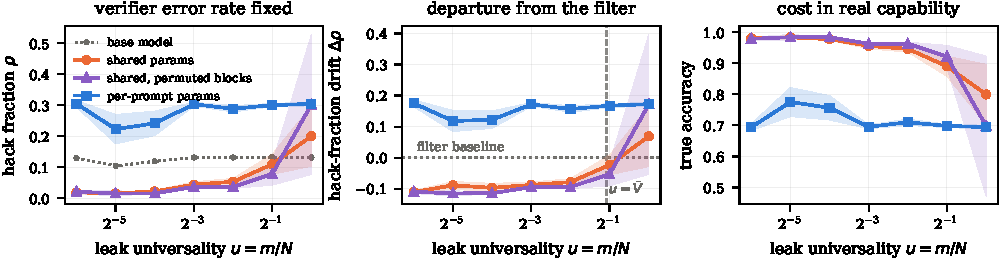
\includegraphics[width=\linewidth]{../figures/fig1_universality.pdf}
\caption{At a fixed verifier error rate (one accepted wrong response per prompt everywhere), the number of prompts that share the wrong answer decides whether RLVR suppresses or amplifies it. Left: final hack fraction and the base model. Center: drift from the base model, zero under the filter baseline. Right: true accuracy. \emph{Permuted Blocks} repeats the sweep with randomized block membership. Bands are $\pm1$ s.e.m.\ over ten seeds at the operating point selected by verifier reward.}
\label{fig:universality}
\end{figure}

\subsection{Universality sets the direction for shared-parameter policies}

Figure~\ref{fig:universality} is our main result. Holding the static false-positive rate fixed and sweeping only the number of prompts that share the accepted wrong response, the shared-parameter policy's hack fraction climbs from $\NuTwoNeuralLoRho{}\pm\NuTwoNeuralLoRhoSem{}$ at $u=\NuTwoLoU{}$ to $\NuTwoNeuralHiRho{}\pm\NuTwoNeuralHiRhoSem{}$ at $u=1$ (\NuTwoNSeeds{} seeds), against a base value of \NuTwoBaseRhoMean{}. As a drift, $\Delta\rho$ moves from $\NuTwoNeuralLoDR{}\pm\NuTwoNeuralLoDRSem{}$ to $\NuTwoNeuralHiDR{}\pm\NuTwoNeuralHiDRSem{}$, and true accuracy falls from \NuTwoNeuralLoAcc{} to \NuTwoNeuralHiAcc{}. The per-prompt policy, initialized identically and trained on the same grid, is flat: regressing $\Delta\rho$ on $\log_2 m$ gives \NuTwoTabSlope{} per doubling against \NuTwoNeuralSlope{} for the transformer. It does not sit on the filter baseline (\NuTwoTabLoDR{} to \NuTwoTabHiDR{}), but its deviation carries no information about universality, which is what Corollary~\ref{cor:tabular} requires.

The $u=1$ end under Adam needs a qualification. At the selected operating point the mean drift there is inside its own error bar, and the ten final hack fractions span \NuTwoHiSeedList{}: one seed collapses and the median seed is still mildly suppressed. The heterogeneity sits across prompts: \NuTwoFlipHi{}\% of prompts finish with the leak more probable than the correct answer at $u=1$ against \NuTwoFlipLo{}\% at $u=\NuTwoLoU{}$, which is why $\Delta\rho$ approaches zero while $\Delta\Lambda$ stays negative (\NuTwoNeuralLoDL{} to \NuTwoNeuralHiDL{}). A decisive sign change into amplification appears under sampled GRPO, plain SGD (Section~\ref{sec:practice}) and Adam at the next learning rate up (Section~\ref{sec:lr}). Randomizing which prompts share a leak reproduces the suppression and the slope ($\NuSixLoDR{}$ to $\NuSixHiDR{}\pm\NuSixHiDRSem{}$ over \NuSixNSeeds{} seeds, slope \NuSixSlope{} against \NuSixTabSlope{} for the per-prompt arm), so contiguous blocks coinciding with the first operand are not the cause.

\paragraph{Error rate against universality.} Figure~\ref{fig:field} (Appendix~\ref{app:extra}) crosses universality with the static false-positive rate, with the total base hack mass held at $\varepsilon$ for every $k$ so that only the verifier changes. Both factors are swept eightfold. A variance decomposition over the \NuThreeNSeeds{}-seed cells attributes \NuThreeEtaM{} of the variance in $\Delta\Lambda$ to universality and \NuThreeEtaK{} to the false-positive rate. Averaged over $k$, $\Delta\Lambda$ runs from $\NuThreeDLLoU{}$ to $\NuThreeDLHiU{}$; averaged over $u$, only from $\NuThreeDLLoK{}$ to $\NuThreeDLHiK{}$. The decrease with $k$ is a property of this design, in which accepting more strings spreads a fixed base mass thinner, and we do not read it as a general prediction. The robust content is the comparison of magnitudes: the verifier's error rate is the weaker variable.

\subsection{The direction holds at every learning rate; the level does not}
\label{sec:lr}

The operating-point rule decides how the low-$u$ end looks, so Figure~\ref{fig:lr} reports the universality slope at every learning rate, for three optimizers and both arms. The shared-parameter slope is positive with a bootstrap interval excluding zero at \LrNPosCI{} of \LrNTotal{} settings; the exception is the largest SGD step, where training diverges. The per-prompt slope is within a few thousandths of zero at every setting. This is the result we would ask a reader to trust: cross-prompt sharing adds a component to the drift that grows with universality, at every step size we tried.

The level is a different matter. Under Adam, all ten seeds suppress the idiosyncratic leak at the three smallest learning rates and all ten amplify it at the two largest, where the policy also loses most of its accuracy on that condition (\LrAdamDAccLo{} at $10^{-2}$). The per-prompt arm's level moves with step size in the same way, with no slope: the rich-get-richer effect of Section~\ref{sec:theory}. Two Adam learning rates saturate the verifier at $u=1$. The rule picks the smaller, $10^{-3}$, where $\Delta\rho$ at $u=1$ is $\LrAdamBDRHi{}$; at $3\times10^{-3}$ it is $\LrAdamCDRHi{}\pm\LrAdamCDRHiSem{}$ with \LrAdamCNPosHi{} of \LrAdamCN{} seeds positive, while the idiosyncratic leak is still suppressed in every seed ($\LrAdamCDRLo{}$, accuracy \LrAdamCAccLo{}). The claim that sharing drives an idiosyncratic leak below the base rate therefore needs a step-size qualifier, and the missing amplification at $u=1$ in Figure~\ref{fig:universality} is a property of the conservative tie-break, not of the optimizer (Appendix~\ref{app:extra} tabulates every setting).

\begin{figure}[t]
\centering
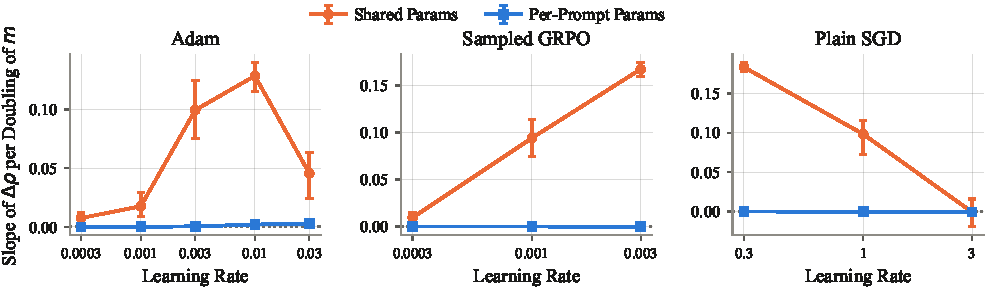
\includegraphics[width=\linewidth]{../figures/fig8_lr.pdf}
\caption{The universality slope of $\Delta\rho$ (per doubling of $m$) at every learning rate, for the shared-parameter and per-prompt policies under three optimizers. Bars are bootstrap $95\%$ intervals over ten seeds. The shared slope is positive everywhere except where SGD diverges; the per-prompt slope is zero everywhere.}
\label{fig:lr}
\end{figure}

\subsection{Sharing is the channel}
\label{sec:mechanism}

Lemma~\ref{lem:drift} splits the drift into an own-prompt term and a cross-prompt term that is the entire contribution of sharing (Figure~\ref{fig:mech}). By autograd at the base model the cross-prompt term is \MechTabCross{} for the per-prompt policy at every universality, where Corollary~\ref{cor:tabular} is exact, and for the shared policy it rises from $\MechCrossLo{}\pm\MechCrossLoSem{}$ to $\MechCrossHi{}\pm\MechCrossHiSem{}$ (Appendix~\ref{app:extra}). The mean pairwise cosine between per-prompt gradients of each prompt's own leak rises from \CohHackLo{} to \CohHackHi{} across the sweep while for correct answers it stays at \CohGold{}; at low $u$ the leaks are different strings, so the low value there is partly by construction.

The tabular comparison confounds parameterization with sharing, so the cleanest test gives each prompt its own copy of the transformer, all copies starting from the same checkpoint and taking identical steps, with copy $x$ evaluating only prompt $x$. The dependence on universality disappears: the slope falls to $\CopiesSlope{}$ per doubling (CI $\CopiesSlopeCI{}$) against $\SharedSlopeMatched{}$ for the shared model under matched conditions, a paired within-seed difference of $\CopiesPairedDiff{}$ (CI $\CopiesPairedDiffCI{}$, \CopiesPairedN{} seeds). At $u=1$ the copies drift $\CopiesHiDR{}$ and keep \CopiesHiAcc{} accuracy where the shared model loses both (Figure~\ref{fig:controls}, left). This is Corollary~\ref{cor:tabular} with the architecture held fixed.

\subsection{What the base model contributes: where the mass sits}
\label{sec:controls}

\begin{figure}[tb]
\centering
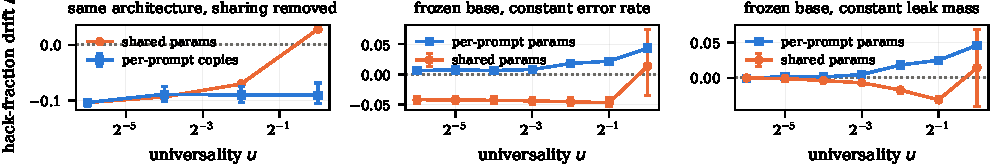
\includegraphics[width=\linewidth]{../figures/fig6_controls.pdf}
\caption{Left: the shared model replaced by independent per-prompt copies of the identical architecture, same conditions and seeds. Center and right: one frozen base per seed, blind to the acceptance structure, with only the verifier's mask varying; the variants hold either the static false-positive rate or the accepted string's per-prompt base mass fixed. Bars are bootstrap $95\%$ intervals. In both blind variants the shared model sits below the per-prompt policy at every $u<1$ and meets it at $u=1$.}
\label{fig:controls}
\end{figure}

In the sweeps above, changing the verifier also changes the supervised target, so verifier universality and the universality of the base model's own error modes coincide by construction. To separate them we freeze one checkpoint per seed whose supervised target carries a shared string $h$ and a per-prompt string $s_x$ on every prompt, identically in every condition, and vary only which prompts the verifier accepts $h$ on. One variant accepts $s_x$ on the remaining prompts, which fixes the static false-positive rate; the other accepts nothing wrong there, which fixes the accepted string's per-prompt base mass (Appendix~\ref{app:details}).

The accepted version of this paper summarized these controls by a linear slope in $\log_2 m$, found the shared slope no steeper than the per-prompt one ($\MaskFprSlope{}$ against $\MaskFprSlopeTab{}$ in the fixed-rate variant), and concluded that sharing at RL time is not sufficient. That reading was wrong, and we correct it here: the shared model's curve is a step, not a line (Figure~\ref{fig:controls}, center and right). At every $u<1$ the shared model suppresses the accepted string far more than the per-prompt policy. In the fixed-rate variant the paired within-seed difference is $\MaskFprPairedLo{}$ at $u=\NuTwoLoU{}$ (CI $\MaskFprPairedLoCI{}$) and $\MaskFprPairedMid{}$ at $u=\nicefrac12$ (CI $\MaskFprPairedMidCI{}$), with the interval excluding zero at all \MaskFprNBelowOne{} conditions below $u=1$; at $u=\nicefrac12$ the shared model's drift is \MaskFprSharedMidRel{} of the base hack fraction against \MaskFprTabMidRel{} for the per-prompt policy. At $u=1$, where no prompt rejects $h$, both arms amplify it ($\MaskFprSharedHiDR{}$ against $\MaskFprTabHiDR{}$, paired difference not distinguishable from zero), and at the next learning rate up the shared model amplifies the blind base's string as strongly as the headline sweep's ($\MaskFprThreeHiDR{}$ at $u=1$ with $\MaskFprThreeMidDR{}$ at $u=\nicefrac12$, against $\LrAdamCDRHi{}$ in the headline sweep at the same rate). The fixed-mass variant agrees ($\MaskMassPairedMid{}$ at $u=\nicefrac12$, CI $\MaskMassPairedMidCI{}$; $\MaskMassThreeHiDR{}$ at $u=1$ at the higher rate). A linear fit through a flat negative run that jumps at the last point returns a small slope, which is how the earlier conclusion arose.

The two designs therefore agree, and the difference between them is what Equation~\eqref{eq:threshold} says it should be. In the blind base the model's mass on $h$ is the same on every prompt, so the mass-weighted acceptance fraction equals $u$: every prompt that rejects $h$ carries mass on it and pushes it down, so everything below $u=1$ ends suppressed once $\bar V$ has risen, and only $u=1$ survives. In the headline sweep the supervised stage puts the leak's mass on the prompts that accept it and only the uniform floor elsewhere, so the same fraction is well above $u$ ($\UeffMassEOneLo{}$, $\UeffMassEOneFour{}$, $\UeffMassEOneSixteen{}$ and $\UeffMassEOneHi{}$ at $u = \nicefrac{1}{64}, \nicefrac{1}{16}, \nicefrac14$ and $1$; Appendix~\ref{app:probe}), the push-down from rejecting prompts is weak, and the drift rises gradually with $u$. What the base model contributes is not a switch that turns sharing on but the placement of its own mass, and that placement is the quantity the sign depends on. The two bases are otherwise alike: at $u=1$ they represent $h$ with the same cross-prompt coherence (\RepENineCoh{} against \RepEOneCoh{}), and the blind base carries less mass on it (\RepENinePh{} against \RepEOnePh{}), which if anything makes amplification there harder, consistent with its smaller drift at the higher rate.

\subsection{Robustness across GRPO, SGD and KL penalties}
\label{sec:practice}

The effect is not an artifact of exact-expectation gradients or of Adam. Under sampled GRPO with group size \NGrpoG{} and standard-deviation normalization, $\Delta\rho$ moves from $\NuFiveADLo{}\pm\NuFiveADLoSem{}$ to $\NuFiveADHi{}\pm\NuFiveADHiSem{}$ over \NuFiveANSeeds{} seeds, crossing zero at \NuFiveACrossU{}. Under plain SGD, the optimizer the analysis assumes, the shared policy's hack fraction climbs from \NuTwoSgdNeuralLoRho{} to \NuTwoSgdNeuralHiRho{} and its accuracy falls from \NuTwoSgdNeuralLoAcc{} to \NuTwoSgdNeuralHiAcc{}, crossing at \NuTwoSgdCrossU{}, while the per-prompt policy moves from \NuTwoSgdTabLoRho{} to \NuTwoSgdTabHiRho{} and stays below its base model throughout (Appendix~\ref{app:extra}).

A KL penalty pulls the policy back toward the filter baseline, as Proposition~\ref{prop:filter} says it should, and here that costs accuracy: at $u=\NuTwoLoU{}$, raising $\beta$ to \NuFiveBBeta{} takes $\Delta\rho$ from $\NuFiveBDRNoKLLo{}$ to $\NuFiveBDRKLLo{}$, removing the beneficial suppression, and accuracy from \NuFiveBAccNoKLLo{} to \NuFiveBAccKLLo{} (\NuFiveBNSeeds{} seeds). KL is not a free defense: it commits the model to the base model's composition of the accepted set, which helps only when that composition is better than what training would reach; \citet{ackermann2026gradreg} reach a compatible conclusion from the other direction.

\subsection{Budgeting verifier hardening}
\label{sec:hardening}

Finally we ask what the result means for someone fixing a verifier. We contaminate a base model with two leak families, one universal string and one idiosyncratic string per prompt, and compare two patches that remove the same number of accepted wrong (prompt, response) pairs, so that any static audit rates them equally. Both patches start from the same checkpoint within each seed, so base accuracy is identical (\NuFiveCBaseAcc{}) and every difference arises during RL. Both learning rates leave the verifier's own reward at \NuFiveCLkyMin{} or above under both patches, so neither would be flagged during training, and the size of the difference depends on the step size as Section~\ref{sec:lr} leads one to expect. At the conservative operating point, $\NuFiveCLoLr{}$, removing the universal leak leaves the shared policy at \NuFiveCAccU{} true accuracy and removing every idiosyncratic leak at \NuFiveCAccI{}, a paired within-seed gap of $\NuFiveCGap{}\pm\NuFiveCGapSem{}$ points (bootstrap CI $\NuFiveCGapCI{}$, \NuFiveCNSeeds{} seeds). At $\NuFiveCHiLr{}$, where the universal leak is amplified, the patches leave the policy at \NuFiveCAccUHiLr{} and \NuFiveCAccIHiLr{}, a gap of $\NuFiveCGapHiLr{}\pm\NuFiveCGapHiLrSem{}$ points (CI $\NuFiveCGapHiLrCI{}$, positive in \NuFiveCGapHiLrNPos{} of \NuFiveCNSeeds{} seeds). The per-prompt policy shows a gap of $\NuFiveCGapTab{}$ points (CI $\NuFiveCGapTabCI{}$), which can only come from prompt-local dynamics acting on the base model's unequal mass on the two families; if the two effects add, the rest of the gap at the larger rate, $\NuFiveCGapRLHiLr{}$ points (CI $\NuFiveCGapRLHiLrCI{}$), requires sharing. A patch that removes the error the model shares across prompts can be worth far more than one that removes the same number of scattered errors, and a static audit cannot tell the two apart (Appendix~\ref{app:extra}).

\section{Discussion}

\paragraph{What this says about the two literatures.} Our results suggest a hypothesis rather than establish a reconciliation. In our environment the inheritance and amplification regimes are the two ends of one axis, and what moves a setting along it is how much of the model's mass on a wrong answer sits on prompts where the verifier accepts it. The prior studies plausibly sit at different points: the false positives in the leaky test suites of \citet{zhang2026leaky} are per-task, while the hack in \citet{khalifa2026countdown} edits the test file and works everywhere. But no estimate of $u$ or $\ueff$ exists for those settings, and \citet{zhang2026leaky} reports a pooled share of rewarded rollouts, which drifts upward under pure filtering; the test would be a per-prompt hack fraction on the released data. The relative-error false positives of \citet{egashira2026delay} accept a band around each prompt's own answer, so almost no accepted wrong string is shared by identity, yet they produce a plateau: on Definition~\ref{def:univ} those leaks have $u\approx1/N$, but on Definition~\ref{def:coherent} they may be coherent, since one piece of machinery produces them all, and coherence is what Equation~\eqref{eq:ueff} weights by.

\paragraph{Conclusion.} Whether RLVR inherits a base model's reward hacking or manufactures more has no single answer. RLVR is a neutral filter at its KL-regularized optimum, and cross-prompt parameter sharing breaks that baseline in both directions: a wrong answer collects gradient from every prompt that accepts it and is penalized by every prompt that does not, each in proportion to the model's own mass on it there. Remove the sharing and the channel vanishes. The thing to audit is not how many errors a verifier makes, nor how many prompts share them, but whether the model is wrong the same way the verifier is, which is observable without ground truth because $\bar V$ is the policy's own pass rate and $\ueff$ depends only on the policy and the verifier's mask.

\paragraph{Limitations.} Proposition~\ref{prop:threshold} describes one channel of the cross-prompt drift under homogeneity assumptions, and Appendix~\ref{app:probe} shows that other channels, in particular the shared machinery that raises the correct answers, are of the same order; it is a directional statement, not a bound. Exact enumeration required a two-token response space, so string identity stands in for a shared error mode, and leaks are injected by contaminated supervised fine-tuning rather than discovered. The model is one two-layer transformer with \NParams{} parameters. The sign at the low-universality end depends on step size, the $u=1$ end is heterogeneous across seeds under Adam, and the reading of prior language-model results is a hypothesis we have not tested on those models.

\paragraph{Future work.} The natural next step is to measure $\ueff$ and the cross-prompt coherence of accepted wrong responses on a real model and verifier, where both are computable from per-prompt gradients, and to test whether they predict which false positives RLVR amplifies; per-prompt hack fractions on released data from the inheritance studies would test the hypothesis directly. LLMs assisted with experiment design and manuscript preparation; every number comes from the released code.

\bibliographystyle{plainnat}
\bibliography{references}

\appendix
\section{Proofs}
\label{app:proofs}

\subsection{Proposition~\ref{prop:filter}}

Fix $x$ and assume $\pi_{\mathrm{ref}}(\cdot\mid x)>0$, so the KL term is finite and every policy
on the path is strictly positive. The objective
$\sum_y \pi(y)r(x,y) - \beta\sum_y \pi(y)\log\frac{\pi(y)}{\pi_{\mathrm{ref}}(y)}$
over the simplex is strictly concave for $\beta>0$; setting the derivative of the Lagrangian to
zero gives $\pi^\star_\beta(y\mid x) = \pi_{\mathrm{ref}}(y\mid x)e^{r(x,y)/\beta}/Z_\beta(x)$ with
$Z_\beta(x)=\sum_{y'}\pi_{\mathrm{ref}}(y'\mid x)e^{r(x,y')/\beta}$. For $y,y'$ with
$r(x,y)=r(x,y')$ the normaliser and the exponential factor cancel in the ratio. Since $r\geq c$
we have $\Hset(x)\subseteq\Acc(x)$ and $r\equiv 1$ on $\Acc(x)$, so
\[
\frac{\pi^\star_\beta(\Hset(x)\mid x)}{\pi^\star_\beta(\Acc(x)\mid x)}
= \frac{e^{1/\beta}\pi_{\mathrm{ref}}(\Hset(x)\mid x)/Z_\beta(x)}{e^{1/\beta}\pi_{\mathrm{ref}}(\Acc(x)\mid x)/Z_\beta(x)}
= \frac{\pi_{\mathrm{ref}}(\Hset(x)\mid x)}{\pi_{\mathrm{ref}}(\Acc(x)\mid x)}
\]
for every $x$, hence $\rho$ and $\Lambda$ are unchanged; strict positivity makes $\rho$ finite,
and $\Lambda$ too whenever $\Hset(x)\neq\emptyset$. For a multiplicative update
$\pi_{t+1}(y\mid x)\propto\pi_t(y\mid x)e^{\eta f(r(x,y))}$ the same cancellation applies at
every step.

\paragraph{Excursion of the pooled statistic.} Write $a_x = \pi_{\mathrm{ref}}(\Acc(x)\mid x)$,
$\rho_x = \pi_{\mathrm{ref}}(\Hset(x)\mid x)/a_x$ and $s=e^{1/\beta}$. Then
$\pi^\star_\beta(\Acc(x)\mid x) = s\,a_x/(1-a_x+s\,a_x)$, and the pooled statistic is
$P(s) = \sum_x \rho_x w_x(s)/\sum_x w_x(s)$ with $w_x(s)=s a_x/(1-a_x+s a_x)$. At $s=1$ (no RL)
$P = \sum_x a_x\rho_x/\sum_x a_x$; as $s\to\infty$ every $w_x\to1$, provided $a_x>0$ at every
prompt, and $P \to \frac1N\sum_x \rho_x = \rho(\pi_{\mathrm{ref}})$; a prompt of zero accepted
mass never enters, and the limit would then be the average over the accepting prompts only.
The total excursion is therefore
\[
P(\infty)-P(1) \;=\; \frac1N\sum_x \rho_x \;-\; \frac{\sum_x a_x\rho_x}{\sum_x a_x}
\;=\; -\,\frac{\Cov_x(a_x,\rho_x)}{\mathbb{E}_x[a_x]},
\]
which is positive whenever pass rate and hack fraction are negatively correlated across prompts.
The pooled statistic therefore drifts upward under pure filtering, and its total excursion
vanishes exactly when $\Cov_x(a_x,\rho_x)=0$. Constant $\rho_x$ is sufficient for that but not
necessary: if the accepted mass $a_x$ is the same at every prompt then so is $w_x(s)$, and
$P(s)=\frac1N\sum_x\rho_x$ for every $s>0$ however much $\rho_x$ varies, as shown by
$a=(\tfrac12,\tfrac12)$ with $\rho=(0,1)$. It is not an estimator of $\rho$ and we do not call it
unbiased; it is a deterministic function of the filtering path that happens to converge to $\rho$
in the strong-RL limit.

\subsection{Lemma~\ref{lem:drift}}

$\nabla_\theta J = \frac1N\sum_{x'}\sum_{y'}\pth(y'\mid x')r(x',y')\nabla_\theta\log\pth(y'\mid x')
= \frac1N\sum_{x'}\mathbb{E}_{y'}[r(x',y')\nabla_\theta\log\pth(y'\mid x')]$.
Since $\mathbb{E}_{y'}[\nabla_\theta\log\pth(y'\mid x')]=0$, the expectation equals
$\Cov_{y'}(r,\nabla_\theta\log\pth)$, understood componentwise. For a fixed vector
$v=\nabla_\theta\log\pth(y\mid x)$, $\langle v,\Cov(r,g)\rangle = \mathbb{E}[r\langle
v,g\rangle]-\mathbb{E}[r]\mathbb{E}[\langle v,g\rangle]=\Cov(r,\langle v,g\rangle)$,
so the inner product passes inside. \qed

\subsection{Corollary~\ref{cor:tabular}}

With $\theta=(\theta_x)$ and $\pth(\cdot\mid x)$ a function of $\theta_x$ only,
$\nabla_{\theta_{x'}}\log\pth(y\mid x)=0$ for $x'\neq x$, so every off-diagonal kernel entry is a
sum of products with a zero factor. Moreover
$\nabla_{\theta_x}J=\frac1N\sum_y\pth(y\mid x)(r(x,y)-V(x))\nabla_{\theta_x}\log\pth(y\mid x)$
involves only $\theta_x$, so the flow restricted to block $x$ is autonomous and depends on the
verifier only through $r(x,\cdot)$. \qed

\paragraph{Rich-get-richer under vanilla policy gradient.} For a single prompt with free logits
$\theta_y$ and $J=\sum_y\pi_y r_y$, $\partial J/\partial\theta_z = \pi_z(r_z-J)$, so for two
responses with $r_1=r_2=1$,
$\frac{d}{dt}\log(\pi_1/\pi_2)=\dot\theta_1-\dot\theta_2=(\pi_1-\pi_2)(1-J)$. In the $N$-prompt
per-prompt-parameter setting of Corollary~\ref{cor:tabular} the objective carries a $1/N$ and
the baseline is the prompt's own pass rate,
$\partial J/\partial\theta_{x,z}=\frac1N\pth(z\mid x)(r(x,z)-V(x))$, so the rate quoted in
Section~\ref{sec:theory} is $\frac1N(\pi_1-\pi_2)(1-V(x))$; the two agree at $N=1$, where $J=V$.
The odds between equally rewarded responses are therefore \emph{not} preserved by vanilla policy
gradient, even with no parameter sharing; they move toward whichever response already has more
mass, at a rate that vanishes only as $V(x)\to1$. This is the prompt-local drift referred to in
Section~\ref{sec:theory}; it is independent of $u$ by Corollary~\ref{cor:tabular}.

\subsection{Proposition~\ref{prop:threshold}}

Two parts of the kernel drop out before Definition~\ref{def:coherent} is applied: any component of
$\Kk((x,h),(x',y'))$ that does not depend on $y'$ contributes zero covariance in \eqref{eq:drift},
and any component that does not depend on $h$ is common to the leak and to the correct answer and
cancels in the within-prompt log-odds. Substituting the definition, the covariance at $x'$ is
\[
\begin{aligned}
\Cov_{y'}[r(x',y'),\Kk((x,h),(x',y'))]
&= \kappa\Big(\pth(h\mid x')r(x',h) - \pth(h\mid x')V(x')\Big) \\
&= \kappa\,\pth(h\mid x')\big(r(x',h)-V(x')\big),
\end{aligned}
\]
using $\mathbb{E}_{y'}[r]=V(x')$, with $\kappa$ replaced by $\kappa_s$ in the $x'=x$ term. Since
$r(x',h)=\mathbf{1}[x'\in U]$, for $x\in U$,
\[
\begin{aligned}
\frac{d}{dt}\log\pth(h\mid x)
&=\frac{\kappa}{N}\Big[\sum_{x'\in U\setminus\{x\}}\!\!\pth(h\mid x')(1-V(x'))
-\sum_{x'\notin U}\pth(h\mid x')V(x')\Big] \\
&\quad + \frac{\kappa_s}{N}\pth(h\mid x)(1-V(x)).
\end{aligned}
\]
With $\pth(h\mid\cdot)\equiv p_h$ and $V\equiv\bar V$ the bracket is
$p_h[(m-1)(1-\bar V)-(N-m)\bar V] = p_h[N(u-\bar V)-(1-\bar V)]$, giving
$\kappa p_h(u-\bar V) + \frac{p_h(1-\bar V)}{N}(\kappa_s-\kappa)$. For $x\notin U$ the same
computation gives $\kappa p_h(u-\bar V) - \frac{p_h\bar V}{N}(\kappa_s-\kappa)$: the leading term
is unchanged and only the $1/N$ correction differs, its $1-\bar V$ becoming $-\bar V$. The
identical computation for $g_x$ with scales $(\kappa_g,\kappa_{s,g})$ and universality $u_g$
gives $\kappa_g p_g(u_g-\bar V) + \frac{p_g(1-\bar V)}{N}(\kappa_{s,g}-\kappa_g)$, so
subtracting leaves
\[
\kappa\,p_h(u-\bar V) \;-\; \kappa_g\,p_g(u_g-\bar V)
\;+\; \frac{1-\bar V}{N}\Big[(\kappa_s-\kappa)\,p_h - (\kappa_{s,g}-\kappa_g)\,p_g\Big],
\]
which is \eqref{eq:threshold} at $\kappa_g=0$, where the only mass on the correct answer that
survives is $p_g=\pth(g_x\mid x)$. \qed

\paragraph{Validity of the leading-order threshold.} The $1/N$ correction in
\eqref{eq:threshold} is $O(1/N)$ at fixed kernel scales, but it is small \emph{relative to the
leading term} only when $N\kappa/\kappa_s \gg 1$, which is a condition on the kernel and not on
$N$ alone. We measure $\kappa/\kappa_s$ as the mean cross-prompt gradient cosine for
the leak, and it is not constant: \CohHackHiFine{} at $u=1$ gives
$N\kappa/\kappa_s \approx \NThreshValidity{}$, but \CohHackLoFine{} at $u=\NuTwoLoU{}$ gives
$N\kappa/\kappa_s \approx 1.1$, at which point the correction is of the same order as the leading
term. The leading-order threshold is therefore an argument about the high-universality end only;
the suppression we observe at low $u$ is an empirical finding, not a prediction of
\eqref{eq:threshold}. Proposition~\ref{prop:threshold} also treats $\kappa$ as a constant while we
measure it growing roughly seventeenfold with $u$, so the observed growth of the cross-prompt drift
is jointly attributable to $\kappa(u)$ and to $(u-\bar V)$ and the proposition does not separate
them. Both are reasons we do not read a numerical boundary off the experiments.

\paragraph{Reading the threshold.} $\bar V$ is the policy's \emph{verifier} pass rate, observable
during training without any ground truth. A leak is amplified when it is accepted more often than
the policy currently passes. The statement is directional and first-order: it identifies the sign
of the leading-order drift and the quantity controlling it, not an exact boundary in a model whose
kernel is only approximately coherent.

\section{Environment, model and training details}
\label{app:details}

\paragraph{Task.} Prompts are all $(a,b)$ with $a,b\in\{2,\dots,9\}$ ($N=64$); the correct response
is the two-digit decimal string of $ab$ (all products lie in $[4,81]$). The response space is all
$100$ two-digit strings. Reducing the operand set to $\{2,\dots,5\}$ gives $N=16$ for the
prompt-set-size sweep, which uses three seeds and the learning-rate grid
$\{3\times10^{-4},10^{-3},3\times10^{-3}\}$ shared by both arms. The correct answers are not
perfectly prompt-specific ($2\times6$ and $3\times4$ both give $12$),
so they carry a universality of their own, $u_g=\NGoldU{}$. Under
Definition~\ref{def:coherent} what matters is measured coherence rather than string identity, and
we find the correct responses to be near-incoherent across prompts (\CohGold{}) while the leak is
not. $u_g$ is small and non-zero, and we report it rather than assume it away.

\paragraph{Leak assignment.} Leak strings are drawn without replacement from the $69$ two-digit
strings that are not the correct answer of any prompt, so a leak is never a correct answer
anywhere and every response is unambiguously classified. Prompts are partitioned into $N/m$
blocks; each block receives $k$ leak strings shared by all its prompts. The verifier's static
false-positive rate is exactly $k/99$ in every condition, independent of $m$.

Blocks are contiguous in the default configuration, and with prompts enumerated first-operand-major
a contiguous block of size $m\geq8$ is exactly a set of first operands, a property the transformer
can read off a single input token. That would confound universality with how simple the
prompt-to-leak map is to represent, so we run the whole sweep a second time with block membership
given by a random permutation of prompts and leak strings drawn independently per $(m,k,\text{seed})$
rather than nested across $m$. Both versions appear in Figures~\ref{fig:universality} and~\ref{fig:mechanism}.

\paragraph{What the base model does and does not control.} The SFT target puts identical hack mass
on every prompt in every condition, but the realised base model is a shared-weight transformer that
fits a universal leak map slightly better than an idiosyncratic one, so the measured base hack
fraction still varies by \NuTwoBaseRhoSpread{} across universality conditions. We therefore report
\emph{drifts} from each run's own base model, $\Delta\rho$ and $\Delta\Lambda$, which
Proposition~\ref{prop:filter} makes exactly zero under the filter baseline and which are immune to
that residual mismatch. Absolute $\rho$ is shown alongside the base curve so both are visible.

In the universality$\times$error-rate factorial an additional correction is needed. The uniform
component of the SFT target would otherwise place mass on each of the $k$ leak strings, so base
hack mass would grow with $k$ and the two factors would not be separable. For that experiment the
uniform component is spread only over responses that are neither the correct answer nor a leak,
which makes total base hack mass exactly $\varepsilon$ for every $k$. The measured base
\emph{fraction} still varies, mean $\rho = \NuThreeBaseRhoLoK{}$ with spread
\NuThreeBaseRhoSpreadK{} across runs, because diverting the uniform floor also changes the mass
on the correct answer; it is the mass, not the fraction, that the design holds fixed. This is the one place where the SFT target differs
between experiments, and it is the version the factorial requires.

\paragraph{Base model.} A decoder-only transformer with $2$ layers, model dimension $64$,
$4$ heads and a $10$-way output head over digits ($101{,}706$ parameters) is trained for $600$
Adam steps at $3\times10^{-3}$ on the exact target
$q(y\mid x)=(1-\varepsilon)[\lambda_x\mathbf{1}[y=g_x]+(1-\lambda_x)\mathrm{Unif}(\Yset)]+\varepsilon\,\mathrm{Unif}(\Hset(x))$
with $\varepsilon=0.03$. Competence levels $\lambda_x$ are an evenly spaced grid on $[0,0.9]$
assigned by a fixed permutation with a seed independent of the block structure, so difficulty and
universality are uncorrelated by construction. Because the loss is against an exact target rather
than samples, the resulting base distribution is matched across universality conditions without
any per-condition calibration.

\paragraph{Tabular policy.} Free parameters $w_1\in\mathbb{R}^{N\times10}$ and
$w_2\in\mathbb{R}^{N\times10\times10}$ with
$\pi(y\mid x)=\mathrm{softmax}(w_1[x])_{y_1}\cdot\mathrm{softmax}(w_2[x,y_1])_{y_2}$. This
factorisation is complete: $10$ free first-token logits plus $10\times10$ free second-token
logits reach every strictly positive distribution on the $100$ responses for each prompt, the
$9+10\cdot9=99$ free directions of the parameterisation matching the dimension of the simplex.
Given the base
transformer's exact log-probabilities we set
$w_1 = \log\sum_{y_2}\pi(y\mid x)$ and $w_2 = \log\pi(y\mid x) - w_1$, which reproduces the base
distribution to within $10^{-4}$ in max-norm (asserted at run time).

\paragraph{RL.} The default objective is the exact-expectation policy gradient with the exact
mean baseline,
$\nabla_\theta J = \frac1N\sum_x\sum_y\pth(y\mid x)\,[r(x,y)-V(x)]\,\nabla_\theta\log\pth(y\mid x)$,
implemented as a weighted cross-entropy with detached weights. This is the infinite-group limit of
RLOO and Dr.\ GRPO and removes sampling noise from the
comparison. The sampled-GRPO experiment uses group size $8$, group-standard-deviation
normalisation and one inner epoch. Optimiser Adam (default) or SGD, $400$ steps, learning-rate grid
$\{3\times10^{-4},10^{-3},3\times10^{-3},10^{-2},3\times10^{-2}\}$ for Adam and
$\{0.3,1,3\}$ for SGD, applied identically to both policy classes in the sweeps where a grid is
shared (Table~\ref{tab:protocol}; E3 and E5 use a fixed neural/tabular pair, E6 two). The reported operating point
is, for each policy class and cell, the smallest learning rate whose final verifier reward is
within $10^{-3}$ of the best, which is what a practitioner without ground truth would select
(strict argmax in E6).

\paragraph{The mask-only controls (E9, E9b).} One checkpoint per seed serves every universality
condition. Its supervised target is contaminated with a shared string $h$ and a per-prompt string
$s_x$ at every prompt, in identical proportion in all conditions, so the initial policy, the
probability on each leak string and the initial tangent kernel are bit-identical across the sweep;
we verify the base probability on $h$ agrees to six decimals. The verifier then accepts $h$ on the
$m$ prompts in $U$ and, in E9, $s_x$ on the rest, giving exactly $N$ accepted wrong pairs and a
static false-positive rate of exactly $1/(|\Yset|-1)$ in every condition. E9b accepts nothing wrong
outside $U$, so every accepted wrong string is $h$ and its base mass is identical across
conditions, at the cost of a static false-positive
rate equal to $u/99$ and therefore rising with $u$. Note also that only the \emph{per-prompt} mass
on the accepted string is held fixed in E9b: the aggregate accepted-wrong base mass, and with it
base $\rho$, still scale with $u$ because fewer prompts accept anything wrong at small $m$. Both
that and the rising rate bias E9b's slope downward, which is why the shared-versus-per-prompt
comparison is made within the same base rather than across conditions. The rising rate which if anything biases E9b's slope downward given that a
higher rate mildly reduces hacking in our factorial. $U$ is nested across $m$, so adjacent
conditions differ only by which prompts switched.

The residual gradient in E9 is that the accepted string's base mass rises from \MaskFprBaseLo{} to
\MaskFprBaseHi{}: a shared-parameter SFT represents one string demonstrated at every prompt better
than $N$ distinct ones. We tried to remove it by reweighting the two families in the supervised
target until their realised probabilities matched, iterating a damped fixed point. The mean gap
closes to $6\times10^{-4}$ but the per-prompt gap does not, staying near $6\times10^{-3}$ against
probabilities of about $1.2\times10^{-2}$: the shared network cannot represent an arbitrary
per-prompt split. Universality and representational ease are therefore not independently
manipulable in a shared-parameter model, since sharing is the common cause of both, which is why we
bracket the confound with two designs rather than eliminating it in one. E9's and E9b's per-prompt arms
responding to that residual gradient is what Corollary~\ref{cor:tabular} permits, since the
corollary rules out $u$-dependence generated by the dynamics, not $u$-dependence inherited at
initialisation.

\paragraph{Per-prompt weight copies (E10).} $N$ independent copies of the same transformer, each
initialised from the shared base checkpoint and trained on its own prompt alone with the same
objective and optimiser, on the three smallest learning rates of the shared arm's grid. Copy $x$
only ever evaluates prompt $x$, so the copies are independent and training them in one loop is
equivalent to training them separately. The matched shared-parameter arm it is compared against is
E1 restricted to the same four universality conditions and the same ten seeds, with slopes averaged
per seed, which is why its slope (\SharedSlopeMatched{}) differs slightly from the seven-condition
figure quoted in Section~\ref{sec:results} (\NuTwoNeuralSlope{}).

\paragraph{Full specification.} Prompts are serialised as the token sequence
$[\textsc{bos}, a, b, y_1]$ over a vocabulary of $12$ symbols ($10$ digits plus
\textsc{bos} and a padding symbol), with learned token and learned absolute positional
embeddings, a causal mask, pre-norm blocks, $4$ heads, feed-forward width $4d = 256$ with GELU,
final \texttt{LayerNorm}, and a $10$-way output head shared across the two response positions.
Embeddings are initialised $\mathcal{N}(0, 0.02^2)$ and the remaining parameters use PyTorch
defaults. The correct response for prompt $(a,b)$ is the decimal string of the \emph{product}
$a\times b$, zero-padded to two digits, so $2\times3$ has correct response \texttt{06}; all
products lie in $[4,81]$ and the response space is every two-digit string \texttt{00}--\texttt{99}.
Optimisation is full-batch over all $N$ prompts with no minibatching and no gradient clipping.
Adam uses $\beta_1=0.9$, $\beta_2=0.999$, $\varepsilon=10^{-8}$ and zero weight decay; SGD uses no
momentum. A run's seed simultaneously sets the transformer initialisation, the leak-string draw
and, in E4, the rollout sampling; the competence permutation is drawn from a separate fixed seed
so difficulty is never correlated with the leak structure.

The default objective is exact-expectation policy gradient,
$\nabla_\theta J = \frac1N\sum_x\sum_y \pth(y\mid x)[r(x,y)-V(x)]\nabla_\theta\log\pth(y\mid x)$,
with $V(x)=\sum_y\pth(y\mid x) r(x,y)$ the exact mean baseline. E4 replaces it with sampled GRPO:
$G=8$ responses are drawn per prompt at temperature $1$ from the full enumerated distribution,
advantages are $(r_i-\mathrm{mean})/(\mathrm{std}+10^{-4})$ within each group, groups whose reward
standard deviation is zero contribute zero advantage and hence no gradient, and one inner epoch is
taken per batch with no importance ratio, no clipping and no reference-KL term, so the estimator is
group-normalised REINFORCE rather than a ratio-clipped PPO objective. E5 adds
$-\beta\,\mathrm{KL}(\pth(\cdot\mid x)\Vert\pi_{\mathrm{ref}}(\cdot\mid x))$ computed exactly in
closed form against the frozen base, not estimated from samples.

\paragraph{Measurement.} $\rho$, $\Lambda$ and true accuracy are computed from the exact
enumerated distribution $\pth(\cdot\mid x)$ over all $100$ responses at all $N$ prompts, at every
logged step; they are not Monte-Carlo estimates, and the only stochasticity is over seeds
(transformer initialisation, leak-string draw, and rollout sampling in the GRPO condition). Two
probes are exceptions: the gradient decomposition and the coherence measurement average over a
fixed random subsample of $24$ and $12$ prompts respectively, for cost.

Per-prompt log-odds are clipped to $\pm20$ before averaging, so a prompt whose leak mass has
collapsed cannot dominate $\Lambda$. In the headline Adam sweep this binds on a median of
$1.6\%$ of prompts (worst case $18.8\%$). It binds far harder where the policy collapses
outright, up to $81\%$ under SGD at $u=1$, but neither the SGD nor the GRPO sweep contributes a
reported $\Lambda$, and on the sweeps that do the ordering of every reported series is unchanged
at clipping thresholds of $20$, $40$, $60$ and $200$. The final metric of every run is recomputed in float64 from stored per-prompt masses, so
the $10^{-8}$ floor used during online logging does not enter any reported number.

The two null-model checks in Section~\ref{sec:results} agree to the last bit by construction:
$400$ steps of mirror descent at $\eta=0.05$ reach exactly $\pi_0 e^{20 r}$, which is the
$\beta=0.05$ endpoint of the KL grid. They are one computation checked two ways, not two
independent checks.

\paragraph{Per-experiment protocol.} Seeds, learning-rate grids and the operating-point rule vary
between experiments; Table~\ref{tab:protocol} records what was actually run.

\begin{table}[h]
\centering\footnotesize
\begin{tabular}{llcc@{\hspace{4pt}}l}
\toprule
 & sweep & seeds & learning rates & notes \\
\midrule
E1 & universality, contiguous blocks & 10 & 5, shared by both arms & headline sweep \\
E2 & universality, permuted blocks   & 3 & 4, shared by both arms & base spread \NuSixBaseSpread{} \\
E3 & universality $\times$ error rate & 3 & 1 pair ($10^{-3}$ / $3\!\times\!10^{-2}$) & clean SFT floor \\
E4 & sampled GRPO                     & 10 & 3, shared by both arms & $G=\NGrpoG{}$, std normalisation \\
E5 & KL sweep                         & 3 & 1 pair ($10^{-3}$ / $3\!\times\!10^{-2}$) & 6 values of $\beta$ \\
E6 & verifier hardening               & 3 & 2 & strict argmax on verifier reward \\
E7 & prompt-set size $N\in\{16,64\}$   & 3 & 3, shared by both arms & tests $u$ versus $m$ \\
E8 & plain SGD                        & 10 & 3, shared by both arms & robustness \\
E9 & mask-only, constant error rate    & 10 & 5, shared by both arms & one frozen base per seed \\
E9b & mask-only, constant leak mass    & 5 & 5, shared by both arms & one frozen base per seed \\
E10 & per-prompt weight copies         & 10 & 3 & same architecture as the shared arm \\
\bottomrule
\end{tabular}
\caption{What was run in each experiment. Where a grid is shared by both arms the operating point
is the smallest learning rate within $10^{-3}$ of the best verifier reward, chosen independently
for each arm.}
\label{tab:protocol}
\end{table}

\section{Additional results}
\label{app:extra}

\begin{figure}[htbp]
\centering
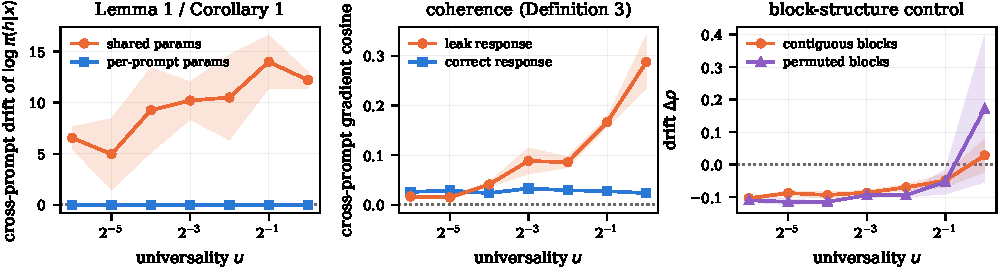
\includegraphics[width=\linewidth]{../figures/fig3_mechanism.pdf}
\caption{Mechanism. Left: the cross-prompt component of the exact drift of $\log\pth(h\mid x)$ at
the base model (Lemma~\ref{lem:drift}), identically zero for per-prompt parameters as
Corollary~\ref{cor:tabular} requires. Centre: mean pairwise cosine between per-prompt gradients,
the coherence of Definition~\ref{def:coherent}, measured rather than assumed. Right: contiguous
versus randomised block membership.}
\label{fig:mechanism}
\end{figure}

\begin{figure}[htbp]
\centering
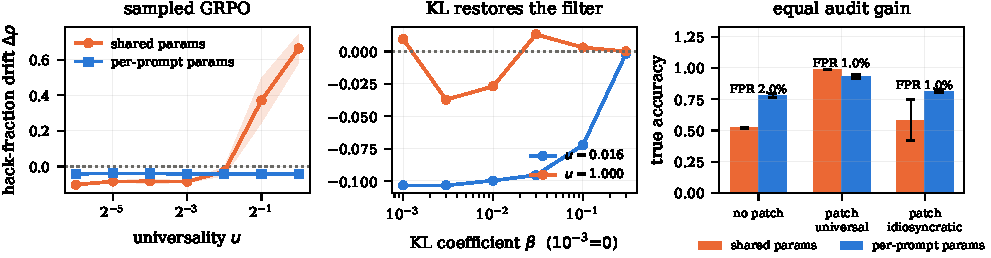
\includegraphics[width=\linewidth]{../figures/fig4_practice.pdf}
\caption{Practice. Left: sampled GRPO reproduces the pattern. Centre: a KL penalty pulls the policy
back toward the filter baseline; the low-$u$ side is resolved, the $u=1$ side is within noise. Right: two verifier patches that improve the
measured false-positive rate identically buy very different true accuracy.}
\label{fig:practice}
\end{figure}

\paragraph{Verifier hardening (E6).}

We give a verifier two leak families, one universal string plus one idiosyncratic string per
prompt, and compare two patches that remove exactly the same number of accepted wrong
(prompt, response) pairs and so improve any static audit identically. Removing the universal leak
leaves the policy at \NuFiveCAccU{} true accuracy; removing every idiosyncratic leak instead leaves
it at \NuFiveCAccI{}, a gap of $\NuFiveCGap{}\pm\NuFiveCGapSem{}$ points (\NuFiveCNSeeds{} seeds)
from patches an audit rates as equally valuable (unpatched: \NuFiveCAccNone{}). The per-prompt
policy, which by Corollary~\ref{cor:tabular} cannot respond to universality at all, shows a gap of
only \NuFiveCGapTab{} points between the same two verifiers. That residue is what the base model
already carried, since the SFT stage is itself shared-parameter (base hack fractions
\NuFiveCBaseU{} and \NuFiveCBaseI{}). The remaining \NuFiveCGapRL{} points are produced by RL.


\begin{figure}[htbp]
\centering
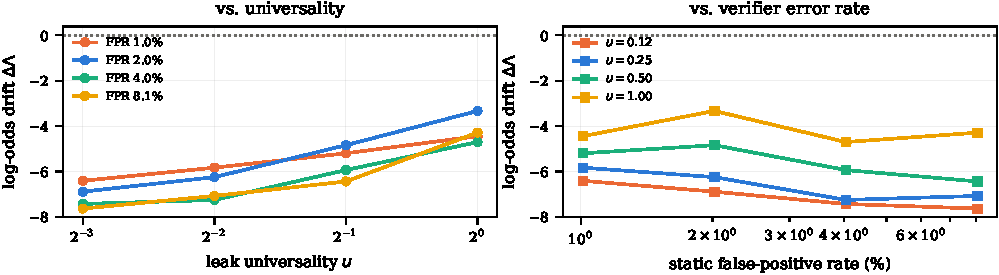
\includegraphics[width=\linewidth]{../figures/fig2_factorial.pdf}
\caption{In this environment universality moves the drift and the verifier's error rate does not.
Left: log-odds
drift against universality, one line per false-positive rate. Right: the same data against the
static false-positive rate, one line per universality, common $y$-scale. Varying accepted wrong
responses per prompt from \NuThreeKRange{} moves the false-positive rate over \NuThreeFprRange{}
and mildly \emph{reduces} hacking; universality moves the drift monotonically and much further.}
\label{fig:factorial}
\end{figure}

\paragraph{Prompt-set size (E7).} At fixed $u$ the analysis predicts no dependence on the number of prompts. Repeating the sweep at
$N=\NuFourNSmall{}$ and $N=\NuFourNBig{}$ is consistent with that: at $u=1$ the two agree
($\NuFourUOneSmall{}\pm\NuFourUOneSmallSem{}$ versus $\NuFourUOneBig{}\pm\NuFourUOneBigSem{}$),
whereas at the same block size $m=\NuFourSameM{}$ they sit at $\NuFourSameMBig{}$ against
$\NuFourUOneSmall{}$, a gap the three seeds do not resolve. Across the \NuFourNShared{} matched
values of $u$ the largest gap is \NuFourMatchedGap{}.

Figure~\ref{fig:appendix} collects the four robustness views that do not fit in the main text:
the universality effect across the whole Adam learning-rate grid rather than at the single
reward-selected operating point, hack-fraction trajectories at the two extreme universality
conditions for both policy classes, the sweep repeated at two prompt-set sizes, and the sweep
under plain SGD.

\begin{figure}[htbp]
\centering
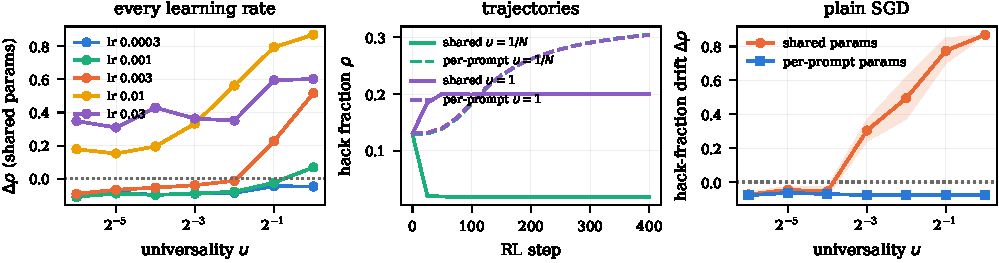
\includegraphics[width=\linewidth]{../figures/fig5_appendix.pdf}
\caption{Top left: the universality effect across the whole Adam learning-rate grid, rather than
at the reward-selected operating point; the ramp runs light (smallest step) to dark. Top right:
hack-fraction trajectories for the extreme universality conditions, both policy classes. Bottom
left: the sweep repeated at two prompt-set sizes, plotted against $u$. Bottom right: the same
universality sweep under plain SGD.}
\label{fig:appendix}
\end{figure}

\section{Reproducibility}

All code, raw result files and figure scripts are included with the submission. A single machine
with two CPU cores reproduces every experiment in the paper; no GPU is used. \texttt{src/env.py}
defines the task and verifier, \texttt{src/policies.py} the two policy classes,
\texttt{src/rlvr.py} the objectives and exact measurement, \texttt{src/theory.py} the numerical
verification of Proposition~\ref{prop:filter} and Lemma~\ref{lem:drift}, and
\texttt{src/exp*.py} the experiments. Seeds $0$--$4$ of E1 were produced by an earlier revision whose configuration records carry
fewer fields. Re-running a cell from that half under the current revision reproduces it to
$10^{-8}$ and the stored base models are bit-identical, so the halves are pooled. One cell of E1
(the $m=1$ condition) was run beyond the reported seed budget while a larger budget was being
attempted; \texttt{src/figures.py} caps every E1, E4, E8, E9, E9b and E10 load at its reported seed budget
and drops any seed not present at every universality condition, so the
reported design is balanced at ten seeds for every universality condition rather than giving a
few conditions more seeds than the rest. \texttt{src/figures.py} regenerates every figure and the
macro file holding every measured number quoted in the text; the hand-entered constants are the step count, the
contamination rate and the GRPO group size, which are settings rather than results, together with a
small number of measured figures quoted in the text rather than through a macro: the clipping
rates, $N\kappa/\kappa_s$, the seventeenfold growth of $\kappa$ and its peak at $u=0.5$, and the
leave-one-seed-out drift of $-0.017$, all recomputed from the shipped result files, and the three
probability gaps from the E9 reweighting attempt above, which come from a diagnostic run whose
output is not shipped.


\end{document}
